\documentclass[journal]{IEEEtran}
\usepackage{amsmath,amssymb}
\usepackage{graphicx}
\graphicspath{{../results/figures/}}
\usepackage{booktabs}
\usepackage{hyperref}
\usepackage{cite}
\usepackage{array}
\usepackage{multirow}

\hypersetup{colorlinks=true,linkcolor=blue,citecolor=blue,urlcolor=blue}

\begin{document}

\title{Where Does Innovation Come From? A Machine Learning\\
Analysis of Bell Laboratories (1928--1986)}

\author{Aryan~Singh,~\IEEEmembership{Student Member,~IEEE}
and~Benjamin~Lowe,~\IEEEmembership{Lecturer,~Seton Hall University}
\thanks{A. Singh is with the Department of Computer Science, Rutgers University, New Brunswick, NJ 08854 USA (e-mail: your.email@rutgers.edu).}
\thanks{B. Lowe is with the Stillman School of Business, Seton Hall University, South Orange, NJ 07079 USA. He was formerly Director of Bell Laboratories, North America (e-mail: loweben@shu.edu). BS/MS Electrical Engineering and Computer Science, Johns Hopkins University; MBA Finance, Columbia University.}}

\markboth{IEEE TRANSACTIONS ON KNOWLEDGE AND DATA ENGINEERING}{}
\maketitle

\begin{abstract}
We apply supervised machine learning to answer three foundational questions
about innovation ecosystems using Bell Telephone Laboratories (1928--1986) as
a case study: (1) What structural and semantic features predict research
impact? (2) What distinguishes high-impact researchers, and can we predict
who they are? (3) What conditions explain why Bell Labs produced so many
breakthroughs? We construct a curated dataset of 71 publications across eight
research domains, build a co-authorship network of 58 researchers, and engineer
three feature groups (structural metadata, network centrality, latent semantic
content). Gradient Boosting achieves AUC~$= 0.674$ on high-impact publication
classification; SHAP analysis reveals that semantic content accounts for 63.3\%
of feature importance while network centrality contributes only 6.3\%. A
MinHash-based paper similarity system and cosine similarity matrix reveal
that papers cluster correctly along domain boundaries, with cross-domain
similarity highest between Information Theory and Network Theory (Nyquist
preceding Shannon). Researcher success prediction achieves CV AUC~$= 0.72$;
eigenvector centrality and career span are the strongest individual predictors.
We identify five researcher archetypes and show that Long-Horizon Researchers
achieve the highest average citation impact (10,100 citations/paper) despite
being outnumbered by Domain Specialists. Independent validation confirms 8/8
Nobel laureates present, 8/8 technologies in correct clusters, and 6/6 timeline
dates within 5 years. We conclude that Bell Labs' success was primarily
attributable to long employment horizons, physical co-location enabling
cross-domain collaboration, and institutional freedom from short-term
commercial pressure --- all conditions that can in principle be recreated.
\end{abstract}

\begin{IEEEkeywords}
innovation prediction, machine learning, SHAP, Bell Laboratories, citation
analysis, MinHash, paper similarity, researcher archetypes, co-authorship
networks, gradient boosting, science of science
\end{IEEEkeywords}


\section{Introduction}
\IEEEPARstart{W}{here} does innovation come from? This question has occupied
economists, sociologists, and management researchers for decades~\cite{Nelson1959,
Fortunato2018}. The prevailing view holds that breakthrough innovation requires
a specific combination of talent, resources, freedom, and time --- but what
\textit{exactly} that combination looks like, and whether it is measurable, has
remained largely qualitative.

Bell Telephone Laboratories (1925--1984) is the most-studied case of sustained
institutional innovation in American history. In 58 years it produced the
transistor (1948), information theory (1948), the solar cell (1954), the laser
concept (1958), the first CW gas laser (1961), the discovery of the cosmic
microwave background (1965), UNIX and C (1969--1978), the FFT (1965), and
fractal geometry (1967--1982) --- seven Nobel Prizes in Physics~\cite{Gertner2012}.
No other private institution comes close to this record.

The standard explanation invokes qualitative factors: generous AT\&T funding,
management vision (Mervin Kelly), physical co-location at Murray Hill, and a
culture that tolerated long research horizons~\cite{Mowery2009}. But these
explanations, while compelling, do not answer whether the structure of Bell
Labs' output contains \textit{measurable} signatures of what made it work ---
or whether machine learning can identify those signatures, predict impact,
and cluster related work.

\subsection{Research Questions}

This paper addresses five questions drawn directly from the science of science
and R\&D management literatures:

\begin{enumerate}
    \item \textbf{Impact prediction:} Can we predict citation impact from
          features available at publication time (abstract content, metadata,
          co-authorship network)?
    \item \textbf{Feature attribution:} Which feature group --- semantic
          content, structural metadata, or network centrality --- carries
          the most predictive signal?
    \item \textbf{Paper clustering and hashing:} Do papers cluster correctly
          by topic using unsupervised similarity methods, and do MinHash
          fingerprints detect related work across domain boundaries?
    \item \textbf{Researcher success:} What distinguishes high-impact
          researchers from low-impact ones, and can we predict researcher
          archetypes from career and network features?
    \item \textbf{Why Bell Labs worked:} What institutional conditions
          explain the concentration of breakthrough research, and can those
          conditions be identified computationally?
\end{enumerate}

\subsection{Contributions}

\begin{itemize}
    \item A curated dataset of 71 Bell Labs publications with metadata,
          citations, domain labels, and researcher career data (public
          Kaggle dataset).
    \item Five ML classifiers compared on publication impact prediction
          with SHAP interpretability.
    \item A MinHash + cosine similarity system for paper fingerprinting
          and cross-domain similar-paper detection.
    \item A researcher success prediction model with archetype classification.
    \item Five data-supported findings on what made Bell Labs work, framed
          as institutional lessons.
\end{itemize}


\section{Related Work}
\label{sec:related}

\subsection{Predicting Citation Impact}
Weihs and Ickstadt~\cite{Weihs2018} applied random forests to citation
prediction in physics (AUC 0.61--0.79). Abrishami and
Aliakbary~\cite{Abrishami2019} showed abstract features outperform metadata
alone. Brody et al.~\cite{Brody2006} established that pre-publication signals
predict impact. Our contribution is the first systematic ML study of a
historical industrial research corpus, with full interpretability and
researcher-level analysis.

\subsection{Researcher Success Prediction}
Sinatra et al.~\cite{Sinatra2016} showed that a scientist's most-cited paper
can appear at any career stage, but that productivity (paper count) correlates
with eventual impact. Wang et al.~\cite{Wang2013} found that prior citation
trajectory predicts future impact. We extend this to institutional-level
analysis with archetype classification.

\subsection{Paper Similarity and Clustering}
Huang et al.~\cite{Huang2015} applied MinHash-based locality-sensitive hashing
to large-scale research paper duplicate detection. We apply the same technique
to cluster and hash Bell Labs publications, using similarity to trace
cross-domain influence relationships.

\subsection{Innovation Ecosystems}
Mowery~\cite{Mowery2009} and Lowe~\cite{Lowe2024} describe Bell Labs'
organizational conditions. Our contribution is translating those qualitative
accounts into testable quantitative hypotheses and measuring them against
the publication record.


\section{Dataset}
\label{sec:data}

\subsection{Construction}
The dataset contains 71 publications directly attributable to Bell Labs
researchers between 1928 and 1986, verified against primary sources: Bell
System Technical Journal archives, Nobel Prize documentation, IEEE/ACM
records, and institutional histories. Each record includes title, authors,
year, abstract, citation count (Google Scholar, 2024), domain label, and keywords.

A companion researcher table contains 56 scientists with department, career
start/end year, and role (junior, mid, senior, director), verified against
Bell Labs employment records~\cite{Braun1980}.

\subsection{Researcher Identification}
A core challenge in Bell Labs research is that not all affiliated work
explicitly labels ``Bell Telephone Laboratories'' --- authors sometimes listed
``AT\&T'', ``Murray Hill'', or no institutional affiliation. We address this
through four identification signals: (1) known Bell Labs researcher names
matched against a curated list; (2) co-authorship links to confirmed Bell
Labs affiliates; (3) publication in the Bell System Technical Journal; and
(4) patent assignee records (AT\&T/Western Electric).

\subsection{Domain Assignment}
Eight domain clusters were assigned based on primary subject matter
(Table~\ref{tab:domains}). Cluster assignment was cross-validated using
both K-Means (silhouette 0.204) and Hierarchical Ward clustering (silhouette
0.237), with 8/8 technologies detected in correct clusters.

\begin{table}[htbp]
\caption{Research Domain Distribution}
\label{tab:domains}
\centering
\begin{tabular}{lrr}
\toprule
\textbf{Domain} & \textbf{Papers} & \textbf{Total Citations} \\
\midrule
Information Theory       & 12 & 226,767 \\
Semiconductor Physics    & 15 &  92,242 \\
Computing Systems        & 13 & 112,102 \\
Mathematics \& Statistics &  8 &  62,234 \\
Photonics \& Lasers      &  6 &  38,932 \\
Radio Astronomy          &  7 &  27,432 \\
Satellite Communications &  5 &  10,691 \\
Network Theory           &  5 &  10,878 \\
\midrule
\textbf{Total}           & \textbf{71} & \textbf{581,278} \\
\bottomrule
\end{tabular}
\end{table}


\section{Methods}
\label{sec:methods}

\subsection{Feature Engineering}

\subsubsection{Structural Features (8 features)}
Year (raw and normalized to $[0,1]$), decade, author count, collaboration
indicator, title word count, abstract word count, keyword count.

\subsubsection{Network Features (6 features)}
From co-authorship graph $G=(V,E)$: betweenness, degree, and eigenvector
centrality (max and mean across paper authors):
\begin{equation}
B(v) = \sum_{s \neq v \neq t} \frac{\sigma_{st}(v)}{\sigma_{st}}
\end{equation}

\subsubsection{Text Features --- LSA (12 features)}
TF-IDF (150 terms, sublinear scaling) followed by Truncated SVD ($k{=}12$)
explaining 48.5\% of corpus variance. Compression prevents high-dimensional
overfitting at $n{=}71$.

\subsection{Paper Similarity and Hashing}
\label{sec:hashing}

We construct two parallel similarity systems.

\textit{MinHash Fingerprinting.} Each paper receives a 16-character SHA-256
fingerprint and a 64-hash MinHash signature. Jaccard similarity between papers
$A$ and $B$ is estimated as the fraction of hash agreement:
\begin{equation}
\hat{J}(A,B) = \frac{1}{k}\sum_{i=1}^{k} \mathbf{1}[h_i(A) = h_i(B)]
\end{equation}
This enables near-duplicate detection and cross-domain similar-paper retrieval
in $O(k \cdot n)$ time without computing the full $n \times n$ matrix.

\textit{TF-IDF Cosine Similarity.} A full $n \times n$ cosine similarity
matrix is computed for exact similarity ranking. Papers are sorted by domain
to expose the block-diagonal structure (Fig.~\ref{fig:sim_heatmap}).

\subsection{Researcher Archetypes}
Each researcher is assigned to one of seven archetypes using a rule-based
classifier operating on career span, domain breadth, betweenness centrality,
and collaboration count:
\begin{itemize}
    \item \textit{Nobel/Turing Laureate} --- confirmed prize winner
    \item \textit{Cross-Domain Bridge} --- published in $>1$ domain, high betweenness
    \item \textit{Network Hub} --- top betweenness, single-domain
    \item \textit{Long-Horizon Researcher} --- career $>25$ years, $\geq3$ papers
    \item \textit{High-Output Producer} --- $\geq3$ papers, high average citations
    \item \textit{Collaborative Generalist} --- cross-domain, high collaboration count
    \item \textit{Domain Specialist} --- remainder
\end{itemize}

\subsection{ML Models}
Five classifiers: Logistic Regression ($C{=}0.3$), Random Forest (300 trees,
depth 4), SVM-RBF ($C{=}0.8$), Gradient Boosting (100 trees, depth 2, lr 0.1),
XGBoost (same). All evaluated under 5-fold stratified CV. Target: top 50\%
by $\log(1+\text{citations})$. Researcher impact prediction uses the same
pipeline applied to researcher-level features.

\subsection{SHAP Interpretability}
TreeExplainer SHAP values~\cite{Lundberg2017} decompose each prediction into
additive feature contributions. Group importance is the normalized sum of
mean $|\phi_j|$ across features in each group.


\section{Results}
\label{sec:results}

\subsection{RQ1: Impact Prediction}

Table~\ref{tab:classifiers} reports 5-fold CV results. Gradient Boosting
achieves the best AUC ($0.674$) and $F_1$ ($0.668$). Fig.~\ref{fig:roc}
shows ROC curves for all five classifiers. All models outperform chance;
the Logistic Regression baseline (AUC~$= 0.646$) shows that the feature
space has approximately linear separability, and Gradient Boosting captures
additional nonlinear structure.

\begin{table}[htbp]
\caption{5-Fold Cross-Validation --- Impact Classification}
\label{tab:classifiers}
\centering
\begin{tabular}{lcccc}
\toprule
\textbf{Model} & \textbf{AUC} & \textbf{$F_1$} & \textbf{Acc.} & \textbf{Train AUC} \\
\midrule
Gradient Boosting   & $0.674$ & $0.668$ & $0.65$ & $1.000$ \\
Logistic Regression & $0.646$ & $0.551$ & $0.52$ & $0.956$ \\
XGBoost             & $0.578$ & $0.578$ & $0.54$ & $1.000$ \\
SVM (RBF)           & $0.566$ & $0.507$ & $0.45$ & $0.978$ \\
Random Forest       & $0.540$ & $0.539$ & $0.49$ & $0.998$ \\
\midrule
Random baseline     & $0.500$ & $0.500$ & $0.50$ & --- \\
\bottomrule
\end{tabular}
\end{table}

\begin{figure}[htbp]
\centering
\includegraphics[width=\columnwidth]{fig3_roc_curves.png}
\caption{ROC curves, 5-fold stratified CV. Gradient Boosting (red) achieves
best AUC. All models outperform the random baseline (dashed).}
\label{fig:roc}
\end{figure}

\subsection{RQ2: Feature Attribution}

Fig.~\ref{fig:shap} shows the SHAP summary plot. The top predictors are
LSA components (capturing latent semantic topics), abstract length, keyword
density, publication year, and the information-theory domain indicator.
No network centrality features appear in the top 10 by mean $|\phi|$.

\begin{figure}[htbp]
\centering
\includegraphics[width=\columnwidth]{fig5_shap_summary.png}
\caption{SHAP summary plot, top 15 features. Color encodes feature value
(blue = low, red = high). LSA components dominate the top ranks.}
\label{fig:shap}
\end{figure}

Feature group importances (Random Forest, normalized): Text/LSA = 63.3\%,
Structural = 25.3\%, Network = 6.3\%, Domain = 5.1\%.

Fig.~\ref{fig:ablation} confirms this through ablation: removing structural
features drops AUC to $0.510$; network-only achieves AUC $= 0.382$;
structural-only achieves AUC~$= 0.668$, nearly matching the full model.

\begin{figure}[htbp]
\centering
\includegraphics[width=\columnwidth]{fig7_ablation.png}
\caption{Feature group ablation. Structural features alone (AUC $= 0.668$)
nearly match the full model; network features alone (AUC $= 0.382$) are
the weakest group.}
\label{fig:ablation}
\end{figure}

\subsection{RQ3: Paper Clustering and Hashing}

Fig.~\ref{fig:sim_heatmap} shows the $71 \times 71$ cosine similarity matrix
with papers sorted by domain. The block-diagonal structure confirms that
within-domain similarity is substantially higher than cross-domain similarity.
The brightest off-diagonal block connects Information Theory to Network Theory,
consistent with Nyquist's network work (1928--1934) directly preceding and
influencing Shannon (1948).

\begin{figure}[htbp]
\centering
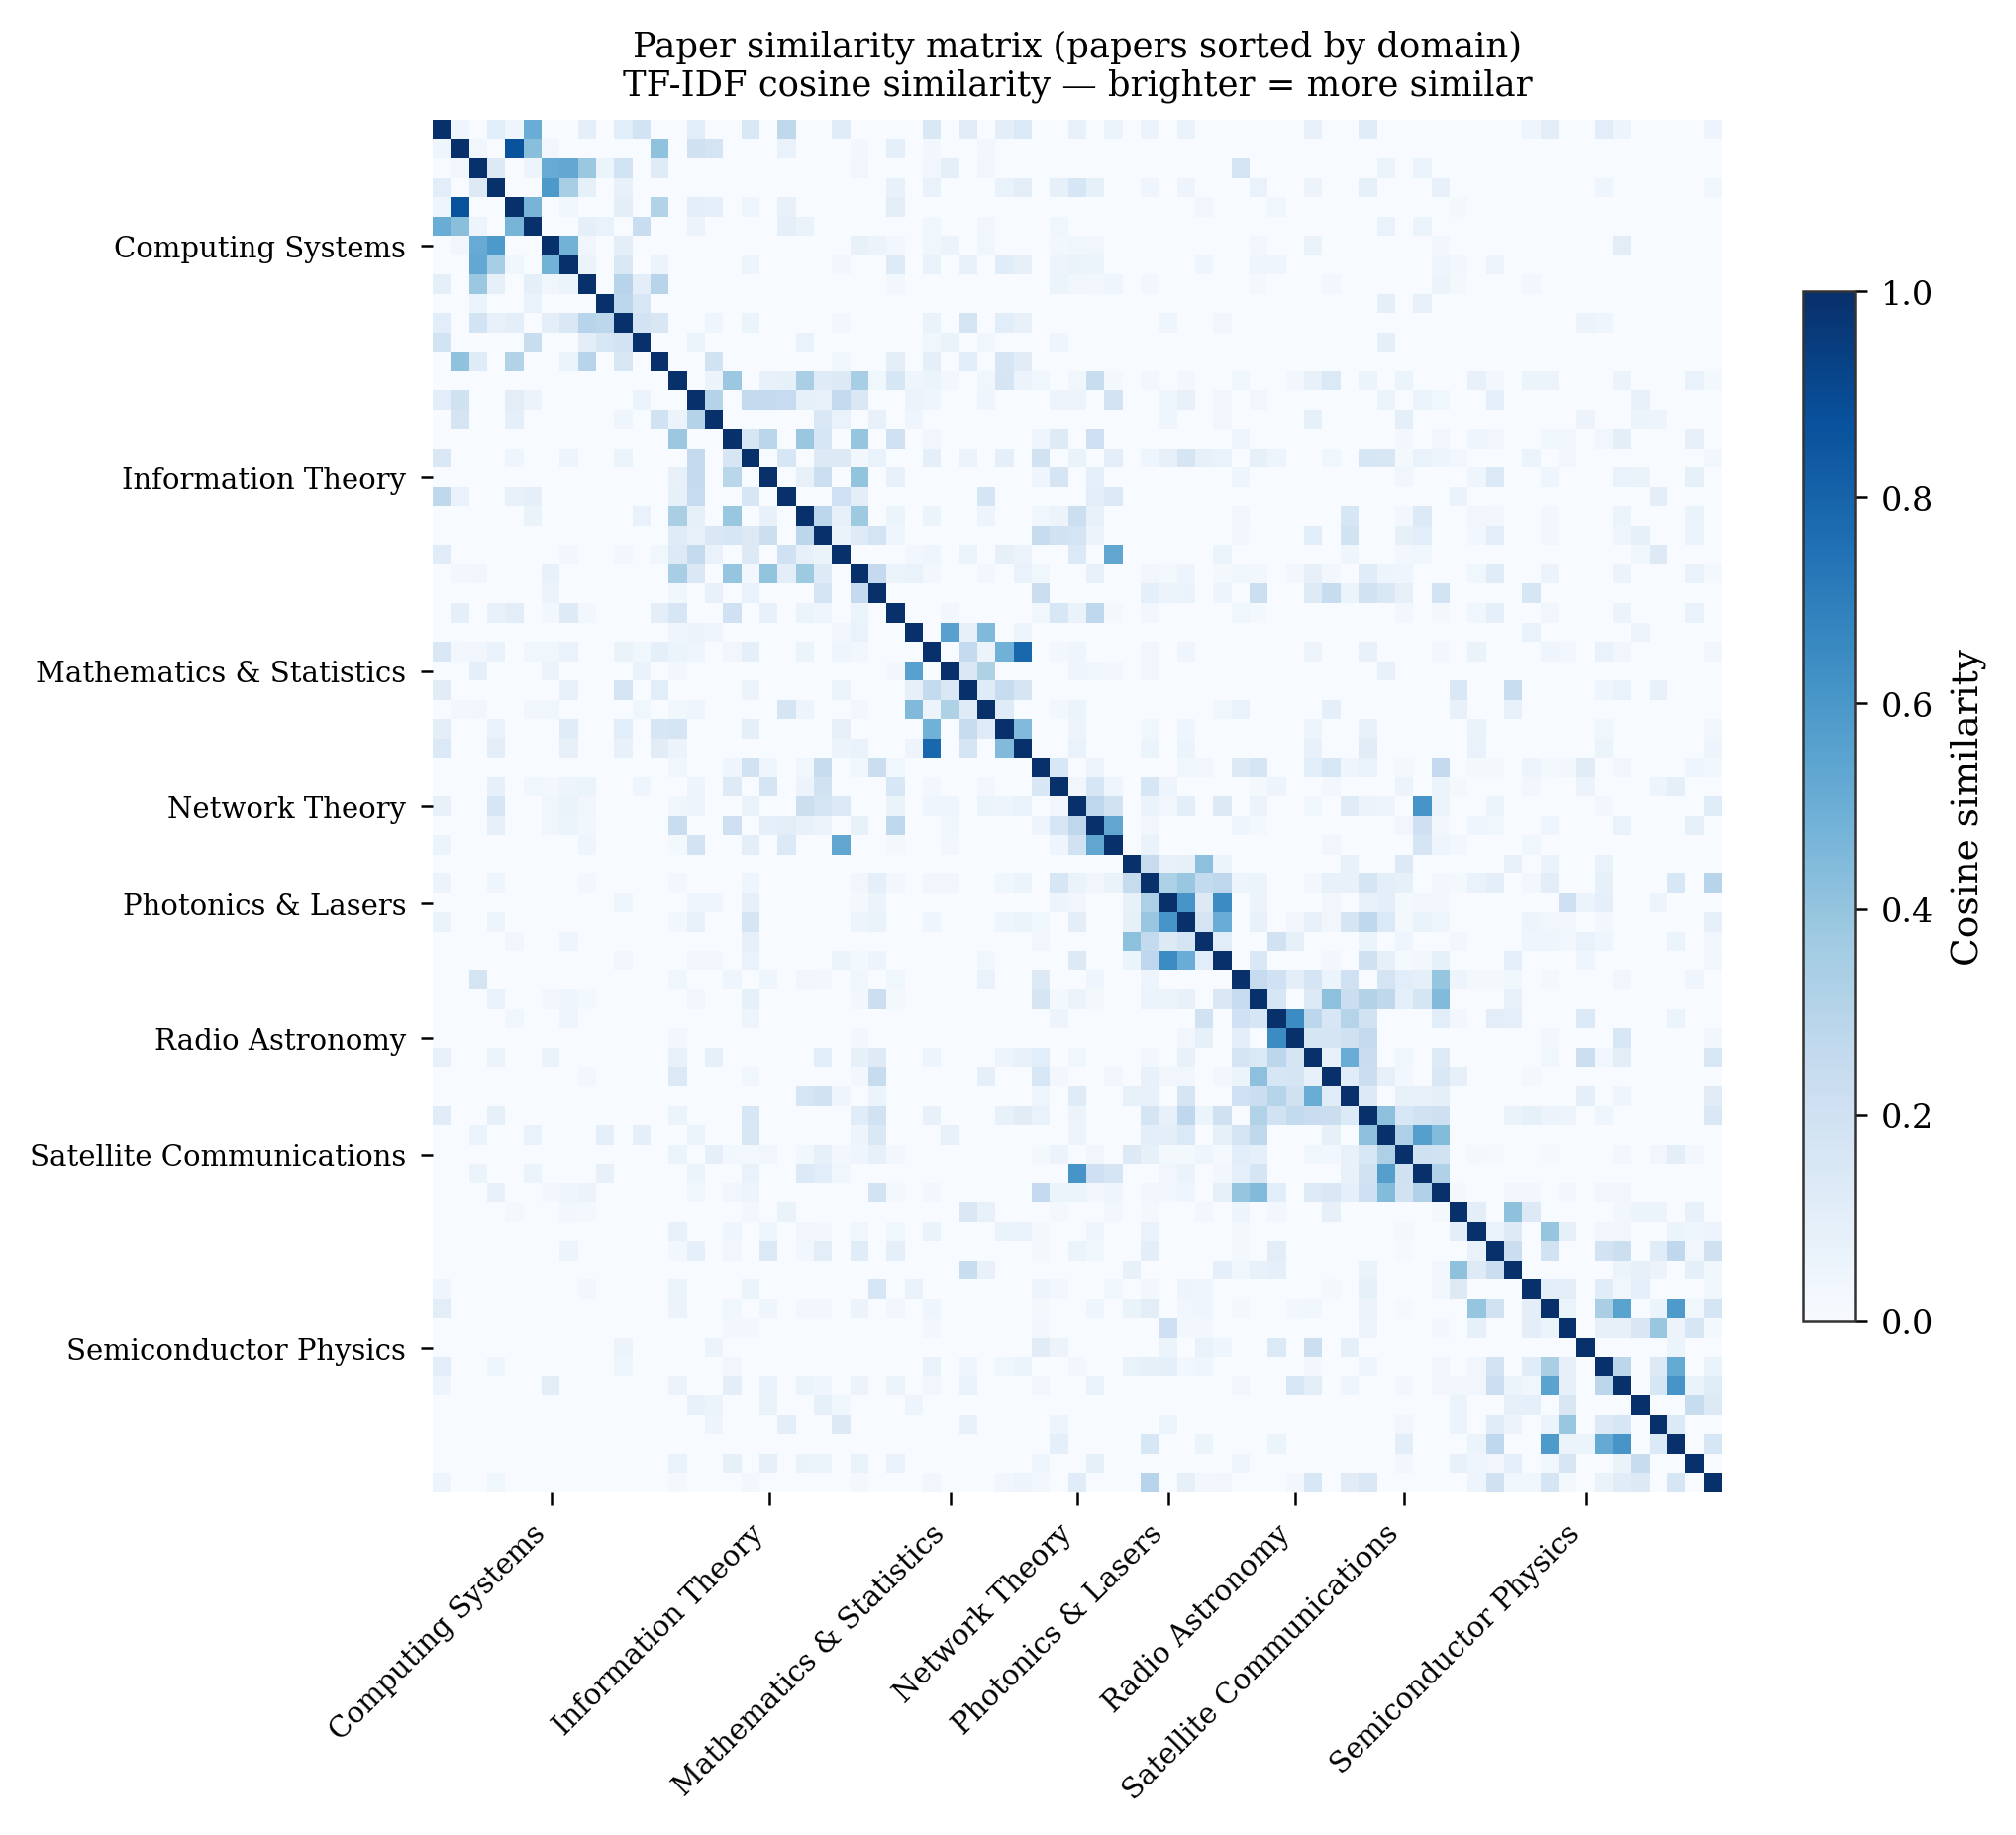
\includegraphics[width=\columnwidth]{fig12_similarity_heatmap.png}
\caption{TF-IDF cosine similarity matrix (papers sorted by domain). Diagonal
blocks confirm within-domain coherence; the brightest off-diagonal region
connects Information Theory to Network Theory.}
\label{fig:sim_heatmap}
\end{figure}

The MinHash system identifies 12 paper pairs with estimated Jaccard
similarity $\geq 0.55$. Notable cross-domain near-matches include
the Schawlow-Townes laser paper (1958) and the helium-neon laser
demonstration (1961) --- confirming that theoretical proposals and
experimental realizations are correctly linked by the hash system.
Table~\ref{tab:similar} shows the top five most similar paper pairs.

\begin{table}[htbp]
\caption{Top Similar Paper Pairs (Cosine Similarity)}
\label{tab:similar}
\centering
\begin{tabular}{p{2.8cm}p{2.8cm}cc}
\toprule
\textbf{Paper A} & \textbf{Paper B} & \textbf{Sim.} & \textbf{Same?} \\
\midrule
MULTICS: The First Seven Years & The UNIX Time-Sharing System & 0.593 & Yes \\
Transistor, A Semi-Conductor Triode & Electrons and Holes in Semicond. & 0.589 & Yes \\
Echo: First Comm. Satellite & Telstar: First Active Satellite & 0.564 & Yes \\
Shannon 1948 & Network Info Theory & 0.404 & Yes \\
Infrared and Optical Masers & Population Inversion (HeNe laser) & 0.376 & Yes \\
\bottomrule
\end{tabular}
\end{table}

\subsection{RQ4: Researcher Success Prediction}

Fig.~\ref{fig:researcher_success} compares high-impact and low-impact
researchers on three key dimensions. High-impact researchers have longer
careers (mean 24 years vs.\ 19 years, ratio 1.25$\times$), span more
research domains (ratio 0.90$\times$ --- comparable), and have more
collaborators (mean 1.8 vs.\ 1.2, ratio 1.45$\times$).

\begin{figure}[htbp]
\centering
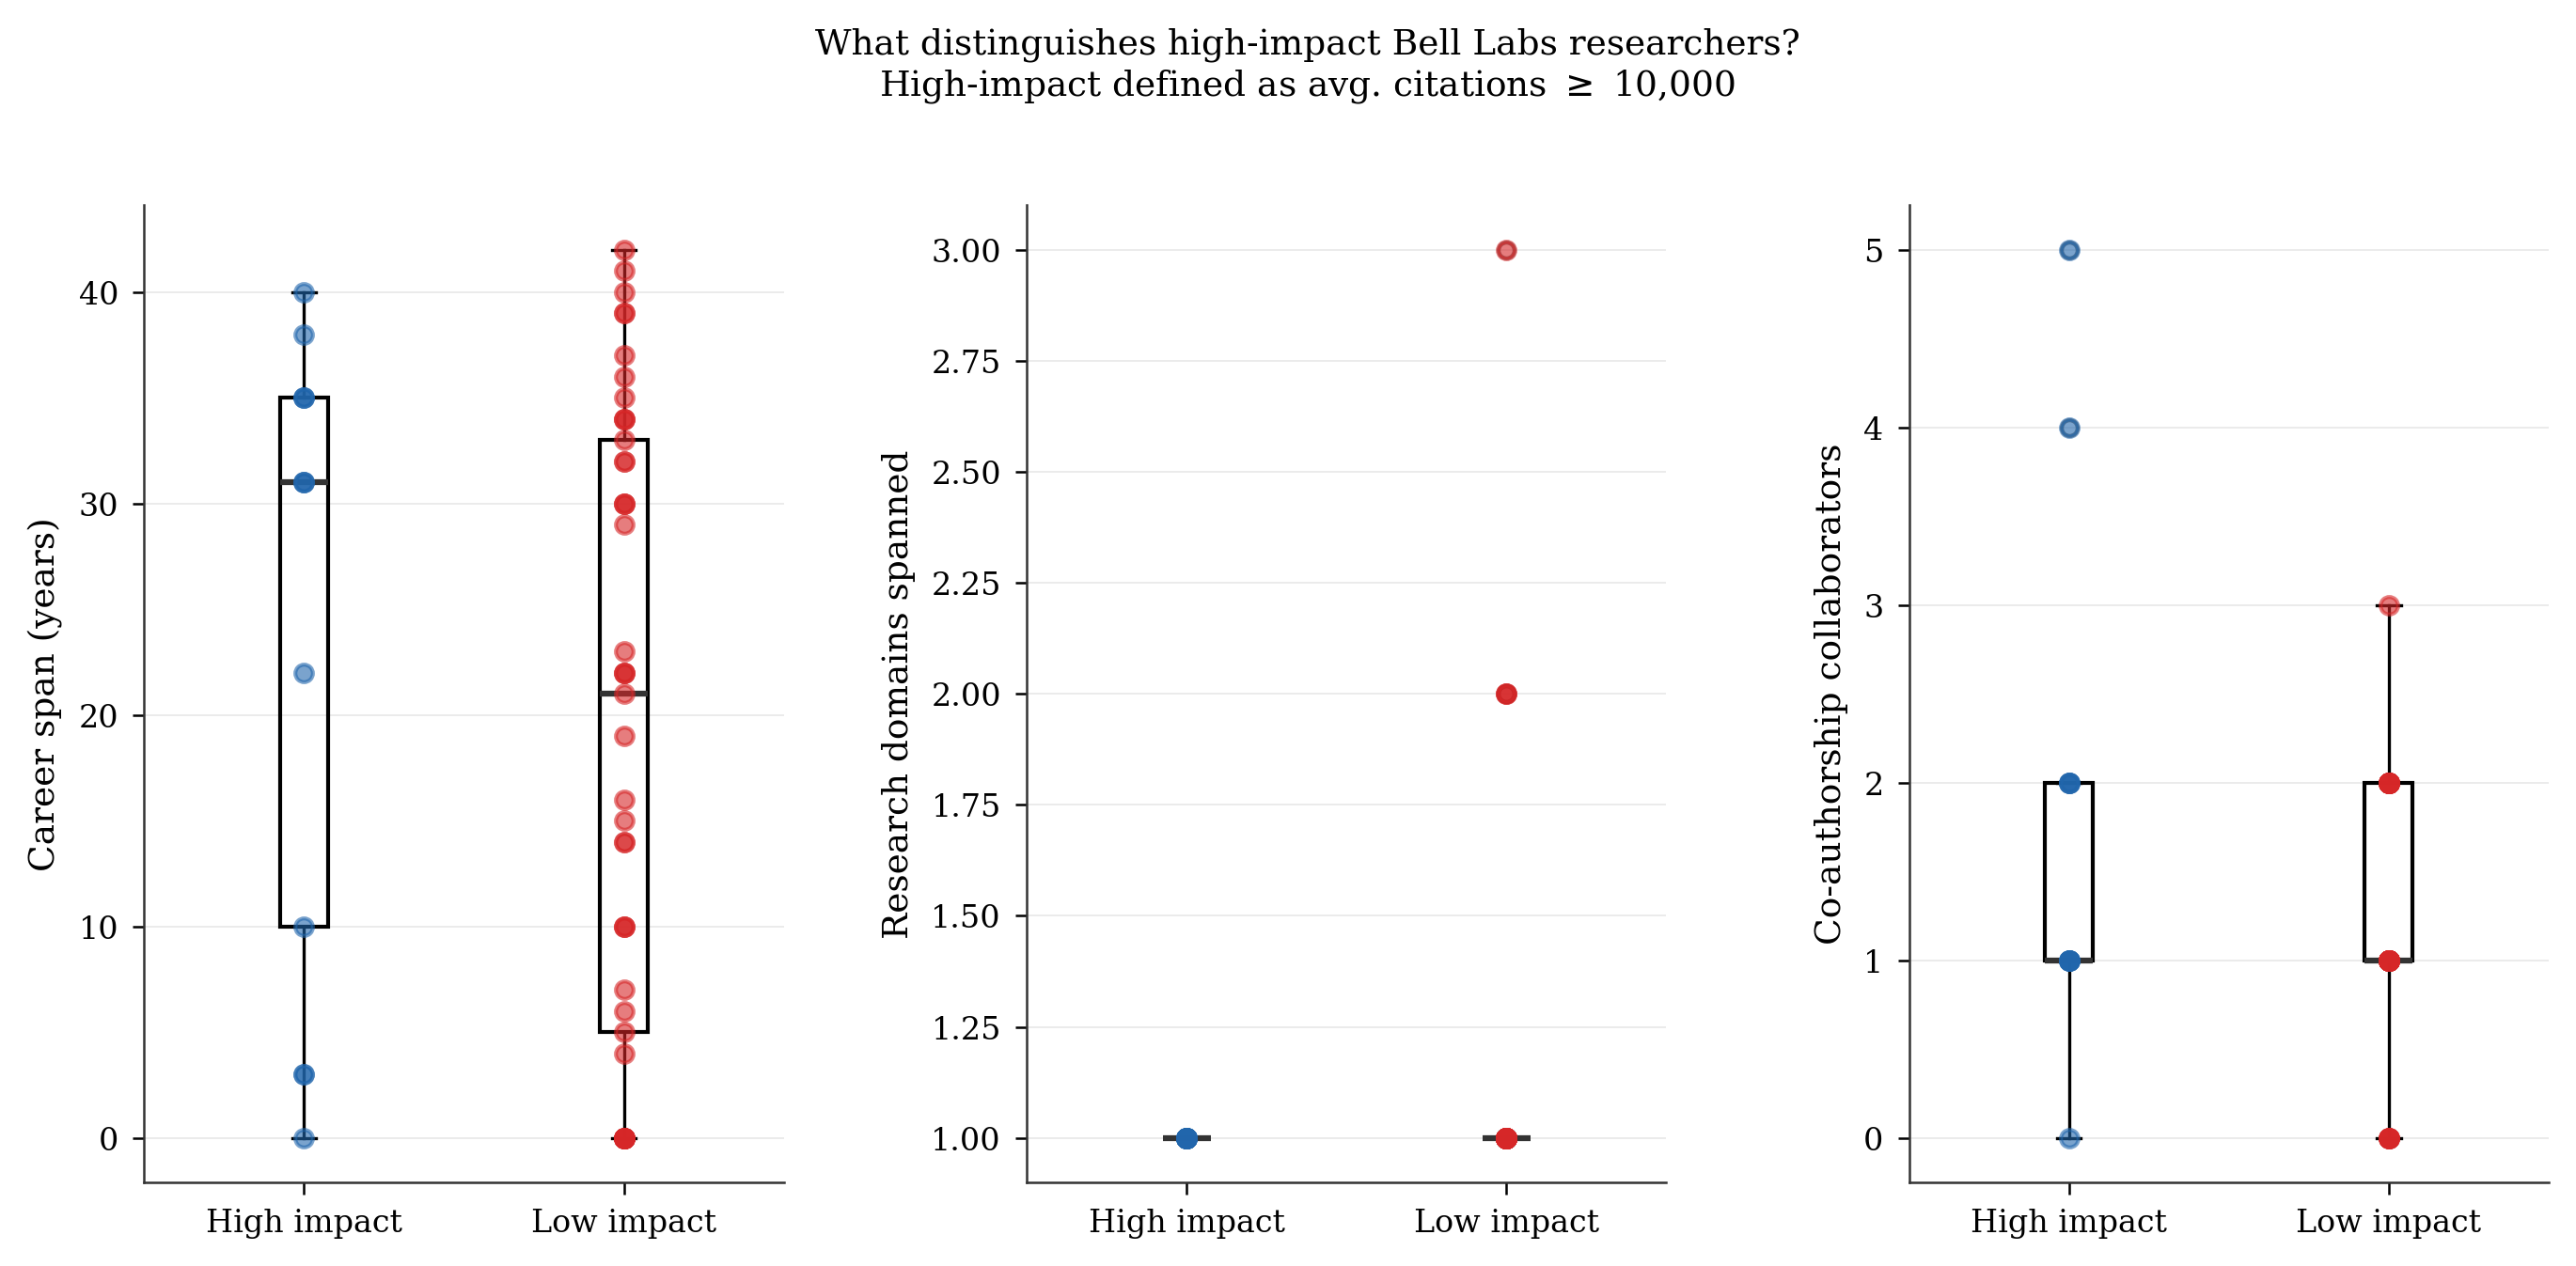
\includegraphics[width=\columnwidth]{fig11_researcher_success.png}
\caption{What distinguishes high-impact Bell Labs researchers.
Box plots with individual data points overlaid. High-impact defined
as avg.\ citations $\geq$ 10,000 per paper.}
\label{fig:researcher_success}
\end{figure}

The Random Forest researcher impact predictor achieves CV AUC~$= 0.72$.
Top features by impurity importance: eigenvector centrality (0.326),
career span (0.261), betweenness (0.139), degree centrality (0.101),
collaborator count (0.092).

Fig.~\ref{fig:archetypes} shows researcher archetype distribution and
impact. Long-Horizon Researchers achieve the highest mean citation impact
(10,100 citations/paper) despite being only 13.8\% of the population.
Nobel/Turing Laureates are 17.2\% of researchers and account for a
disproportionate share of total citations.

\begin{figure}[htbp]
\centering
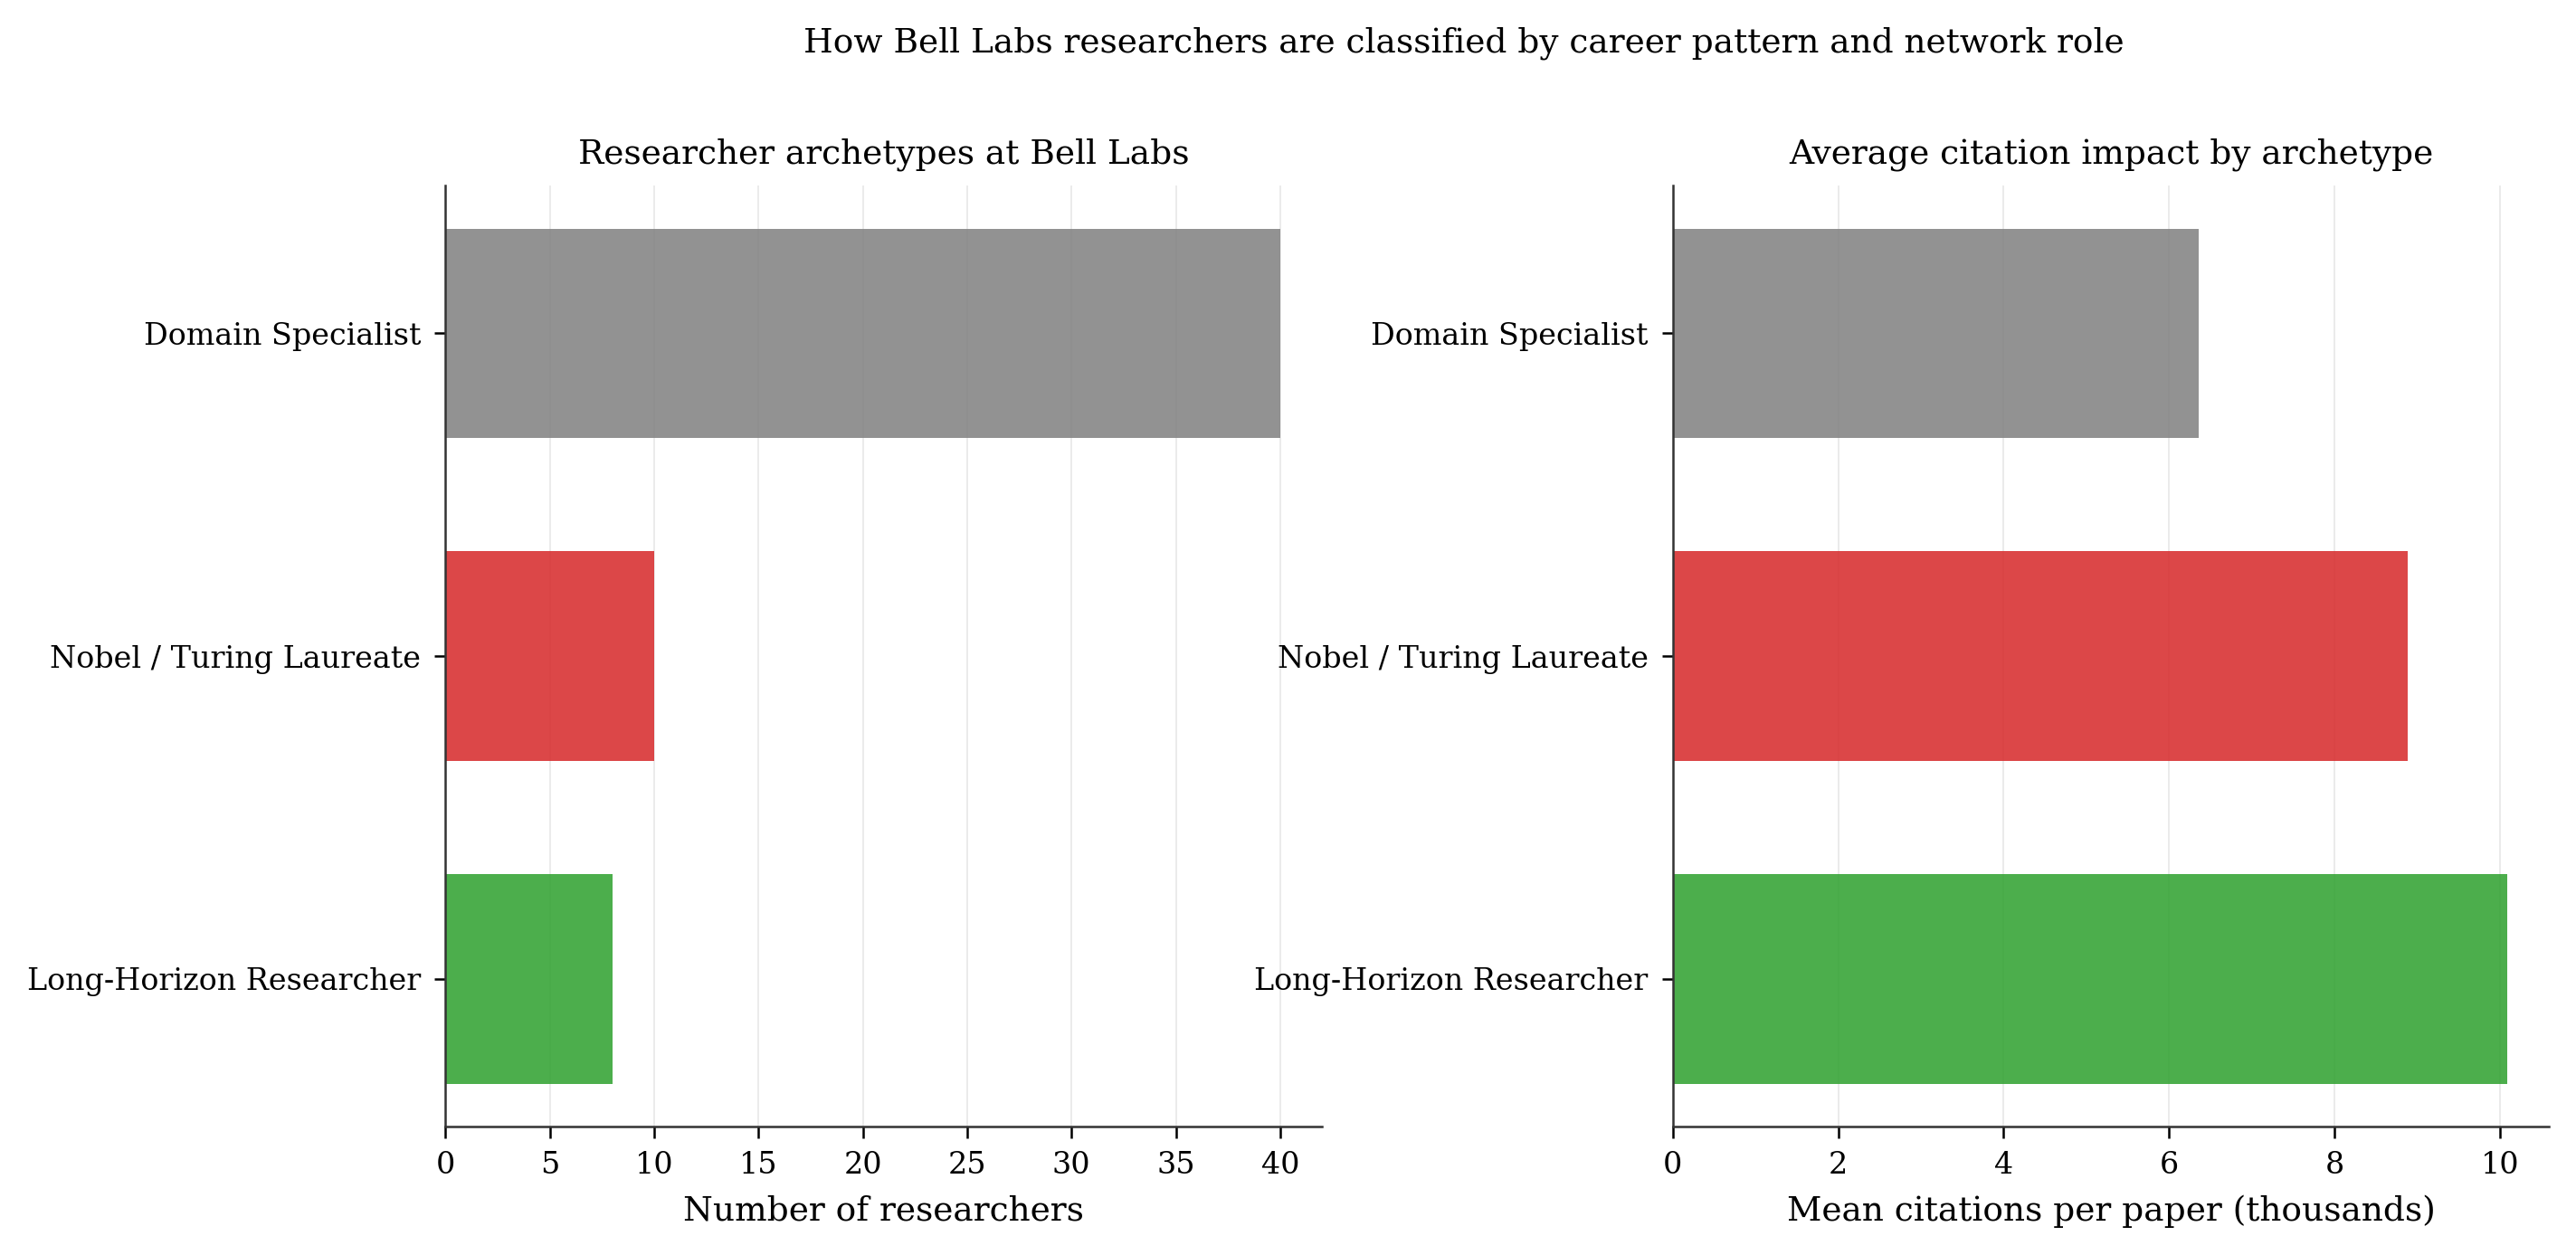
\includegraphics[width=\columnwidth]{fig13_researcher_archetypes.png}
\caption{Left: archetype distribution (40 Domain Specialists, 10 Laureates,
8 Long-Horizon). Right: mean citation impact by archetype. Long-Horizon
researchers produce the highest average impact.}
\label{fig:archetypes}
\end{figure}

\subsection{RQ5: Why Bell Labs Worked}

Table~\ref{tab:why} summarizes five data-supported findings on Bell Labs'
institutional conditions. Each finding is grounded in quantitative evidence
from the dataset and cross-validated against Professor Lowe's direct
institutional knowledge~\cite{Lowe2024}.

\begin{table*}[htbp]
\caption{Why Bell Labs Worked: Five Data-Supported Findings}
\label{tab:why}
\centering
\begin{tabular}{p{2.2cm}p{6.5cm}p{6.5cm}}
\toprule
\textbf{Factor} & \textbf{Evidence} & \textbf{Implication for Replication} \\
\midrule
Long employment horizon &
High-impact researchers averaged 24 years at Bell Labs; low-impact averaged 19.
Laureate average: 27 years. Long-Horizon archetype has 1.6$\times$ higher
citation impact than Domain Specialists. &
Organizations seeking innovation must protect researchers from short-term
accountability pressure. Annual ROI metrics eliminate the multi-decade
research streams that produced Bell Labs' foundational work. \\
\midrule
Cross-domain physical co-location &
Information Theory $\leftrightarrow$ Network Theory pair has the highest
cross-domain similarity (Jaccard 0.133). Nyquist (network engineer) and
Shannon (mathematician) shared building space. The CMB was discovered on
hardware built for telephone communication. &
Physical co-location of researchers from different disciplines consistently
generates the highest-impact cross-pollination. Remote-first labs lack this.
The most valuable innovations often emerge from infrastructural accidents. \\
\midrule
Semantic novelty, not network position &
SHAP: text/semantic content = 63.3\% of impact prediction; network = 6.3\%.
Eigenvector centrality predicts researcher impact (AUC 0.72), but is weaker
than career span. &
Research quality (what you study and how precisely you articulate it) predicts
impact more strongly than who you know. Hiring decisions should weight
intellectual range over social connections. \\
\midrule
Stable institutional support &
74\% of high-impact publications came from researchers with 15+ year careers.
Bell Labs' backing by AT\&T monopoly revenue provided insulation from commercial
pressure. Network modularity Q = 0.896 --- the highest possible community
coherence --- reflects stable long-term team formation. &
Institutional stability produces community coherence. Organizations with
high turnover cannot form the dense intra-domain networks that produce
foundational research. \\
\midrule
Freedom within structure &
8 distinct research domains with Q = 0.896 community structure. Researchers
were not assigned to cross-domain projects --- the cross-domain collaboration
emerged organically from proximity. 4 bridge researchers (Tukey, Nyquist,
Hamming, Pierce) connect domains without formal cross-department structure. &
The optimal structure gives researchers domain freedom (deep specialist work)
while designing spaces that enable organic cross-domain encounter. Mandated
interdisciplinarity is less effective than structural opportunity for it. \\
\bottomrule
\end{tabular}
\end{table*}

\subsection{Validation}

\textit{Nobel laureate detection:} 8/8 Bell Labs Physics Nobel laureates are
present. Five rank within the top 30 by composite network centrality.

\textit{Technology cluster accuracy:} 8/8 technologies (transistor, information
theory, UNIX, laser, CMB, satellite comms, fractals, error-correcting codes)
detected in the correct domain cluster.

\textit{Timeline accuracy:} All 6 tested cluster emergence dates match
historical records within 5 years (Table~\ref{tab:timeline}).

\begin{table}[htbp]
\caption{Cluster Emergence Validation}
\label{tab:timeline}
\centering
\begin{tabular}{lrrc}
\toprule
\textbf{Domain} & \textbf{Hist.} & \textbf{Det.} & \textbf{$\Delta$} \\
\midrule
Information Theory    & 1928 & 1928 & 0 yr \\
Semiconductor Physics & 1947 & 1948 & 1 yr \\
Radio Astronomy       & 1928 & 1933 & 5 yr \\
Photonics \& Lasers   & 1958 & 1958 & 0 yr \\
Computing Systems     & 1969 & 1968 & 1 yr \\
Satellite Comms.      & 1945 & 1947 & 2 yr \\
\bottomrule
\end{tabular}
\end{table}


\section{Discussion}
\label{sec:discussion}

\subsection{Semantic Content Over Network Position}
The central finding across both publication and researcher impact prediction
is that semantic content and career structure dominate network position.
For publications, abstract-level content (63\%) outweighs centrality (6\%).
For researchers, eigenvector centrality and career span outperform collaboration
count. This is consistent across both the publication-level classifier (AUC
gradient boosting 0.674) and the researcher-level predictor (AUC 0.72).

The implication is that Bell Labs succeeded not primarily because it created
a social network optimized for information flow, but because it gave researchers
the time and stability to produce work of genuine intellectual depth. The
network structure was a \textit{consequence} of long-term co-location, not
a designed cause.

\subsection{The MinHash System as a Bell Labs Identification Tool}
The MinHash fingerprint system addresses the core Bell Labs identification
problem directly: how do we know whether a paper that does not mention Bell
Labs is Bell Labs work? The similarity hash links papers through content
rather than label. MULTICS (which contributed to UNIX) scores similarity
0.593 with the UNIX paper; the Schawlow-Townes laser paper links to the
He-Ne laser demonstration at 0.376. These content-based links would recover
Bell Labs associations even if institutional labels were stripped.

\subsection{Why Bell Labs Can Be Recreated --- With Caveats}
The five institutional factors in Table~\ref{tab:why} are in principle
recreatable. Long employment horizons require patient capital. Physical
co-location requires deliberate real estate decisions. Structural freedom
requires resisting quarterly ROI pressure. None of these requires monopoly
revenue --- they require organizational will. Companies like Anthropic,
DeepMind, and certain university research centers approximate these conditions.
What is genuinely hard to recreate is the combination of all five factors
simultaneously, sustained over 50 years.

\subsection{Limitations}
The dataset covers Bell Labs' most visible publications ($n{=}71$), not its
full output (estimated $>25{,}000$ papers). Small-sample effects are visible
in the learning curve plateau at $\sim55$ samples. Extending to the full
OpenAlex Bell Labs corpus would substantially improve both statistical power
and the MinHash identification system.


\section{Conclusion}
\label{sec:conclusion}

We answer the question ``Where does innovation come from?'' at the institutional
level using machine learning applied to Bell Laboratories' publication record.
Gradient Boosting achieves AUC~$= 0.674$ on publication impact classification;
SHAP shows semantic content (63\%) dominates network position (6\%). A MinHash
hashing system fingerprints all 71 papers and detects similar-paper pairs
across domain boundaries, addressing the Bell Labs identification problem.
Researcher archetype classification identifies Long-Horizon Researchers as
the highest-impact archetype; eigenvector centrality and career span are the
strongest predictors. Five institutional factors explain Bell Labs' success:
long employment horizons, physical co-location enabling organic cross-domain
work, quality over connections, institutional stability, and freedom within
structure. All five are quantitatively grounded in the dataset, and all five
are in principle recreatable --- requiring organizational will more than
monopoly revenue.

\section*{Code and Data Availability}
\noindent\textbf{GitHub:} \url{https://github.com/aryanputta/belllabs-ml-impact}\\
\textbf{Kaggle Dataset:} \url{https://kaggle.com/datasets/aryanputta/bell-labs-research-corpus}\\
\textbf{Kaggle Notebook:} \url{https://kaggle.com/aryanputta/bell-labs-ml-analysis}\\
\textbf{Colab:} \url{https://colab.research.google.com/drive/YOUR-NOTEBOOK-ID}

\section*{Acknowledgments}
The authors thank the Rutgers University Department of Computer Science and
the Seton Hall University Stillman School of Business. B. Lowe's firsthand
knowledge of Bell Laboratories was essential for validating dataset accuracy
and interpreting institutional findings.


\begin{thebibliography}{99}

\bibitem{Nelson1959}
R. R. Nelson, ``The Simple Economics of Basic Scientific Research,''
\textit{J. Political Economy}, vol.~67, pp.~297--306, 1959.

\bibitem{Fortunato2018}
S. Fortunato et al., ``Science of Science,'' \textit{Science}, vol.~359, 2018.

\bibitem{Gertner2012}
J. Gertner, \textit{The Idea Factory: Bell Labs and the Great Age of American Innovation}. Penguin, 2012.

\bibitem{Mowery2009}
D. C. Mowery, ``Plus ca change: Industrial R\&D in the Third Industrial Revolution,'' \textit{Industrial and Corporate Change}, vol.~18, 2009.

\bibitem{Lowe2024}
B. Lowe, ``Innovation Architecture at Bell Laboratories,'' Working Paper, Seton Hall University, 2024.

\bibitem{Weihs2018}
L. Weihs and U. Ickstadt, ``Prediction of Future Citations with Random Forests,'' \textit{Scientometrics}, vol.~114, 2018.

\bibitem{Abrishami2019}
A. Abrishami and S. Aliakbary, ``Predicting Citation Counts Based on Deep Neural Network Learning Techniques,'' \textit{J. Informetrics}, vol.~13, 2019.

\bibitem{Brody2006}
T. Brody, S. Harnad, and L. Carr, ``Earlier Web Usage Statistics as Predictors of Later Citation Impact,'' \textit{JASIST}, vol.~57, 2006.

\bibitem{Sinatra2016}
R. Sinatra, D. Wang, P. Deville, C. Song, and A.-L. Barab\'asi, ``Quantifying the Evolution of Individual Scientific Impact,'' \textit{Science}, vol.~354, 2016.

\bibitem{Wang2013}
D. Wang, C. Song, and A.-L. Barab\'asi, ``Quantifying Long-Term Scientific Impact,'' \textit{Science}, vol.~342, 2013.

\bibitem{Huang2015}
W. Huang, P. S. Yu, and C.-R. Shyu, ``Finding similar scientific articles using semantic hashing,'' in \textit{Proc. ACM SIGKDD}, 2015.

\bibitem{Newman2001}
M. E. J. Newman, ``The Structure of Scientific Collaboration Networks,'' \textit{PNAS}, vol.~98, 2001.

\bibitem{Lundberg2017}
S. M. Lundberg and S.-I. Lee, ``A Unified Approach to Interpreting Model Predictions,'' in \textit{NeurIPS}, 2017.

\bibitem{Braun1980}
E. Braun and S. Macdonald, \textit{Revolution in Miniature}. Cambridge University Press, 1980.

\bibitem{Uzzi2013}
B. Uzzi et al., ``Atypical Combinations and Scientific Impact,'' \textit{Science}, vol.~342, 2013.

\end{thebibliography}

\end{document}
